\begin{exercise}
  Describe, in simple sentences with a minimum of mathematical formalism, (1) the score
  of a graph, (2) what the graph score theorem is, (3) the idea of the 
  graph score algorithm, (4) where the difficult part of its proof is.
  Imagine you have a friend who does not take this class, and think about how to answer
  the above questions to them.
\end{exercise} 


\textbf{(1)Conception}
\par At first, we compute every vertex's degree, which means how many other vertices connect to this vertex. Then we sort all degrees from small to large, and this sequence is called as score.
%%%%%%%%%%%%%%%%%%%%%%%%%%%%%%%%%%%%%%%%%%%%%%%%%
\par
\textbf{(2)Theorem}
\par Let $d=(d_1,\cdots,d_n)$ with $d-1\le\cdots\le d_n$. Define $d'$ by
\begin{center}
$$ d_i'=\left\{
\begin{array}{rcl}
d_i-1       &      & {i=n-d_n,\cdots,n-1,n}\\
d_i         &      & {i=1,\cdots,n-d_n-1}\\
\end{array} \right. $$
\end{center}
\par Then there exists a graph with score $d$ if and only if there exist a graph with score $d'$
\par Furthermore, if $n=1$, then there exist a graph with score $(d_1)$ if and only if $d_i=1$.
\par
%%%%%%%%%%%%%%%%%%%%%%%%%%%%%%%%%%%%%%%%%%%%
\textbf{(3)Idea of Algorithm}
\par find-graph $(d_1,d_2,\cdots,d_n)$
\par sort$(d_1,d_2,\cdots,d_n)$
\begin{center}
$$ d_i'=\left\{
\begin{array}{rcl}
d_i-1       &      & {i=n-d_n,\cdots,n-1,n}\\
d_i         &      & {i=1,\cdots,n-d_n-1}\\
\end{array} \right. $$
\end{center}
\par $G'=$ find-graph$(d_1',d_2',\cdots,d_{n-1}')$
\par if $G'=$ NULL
\par return NULL
\par else $G=G'+vertex(n)$
\begin{figure}[hpbt]
\begin{center}
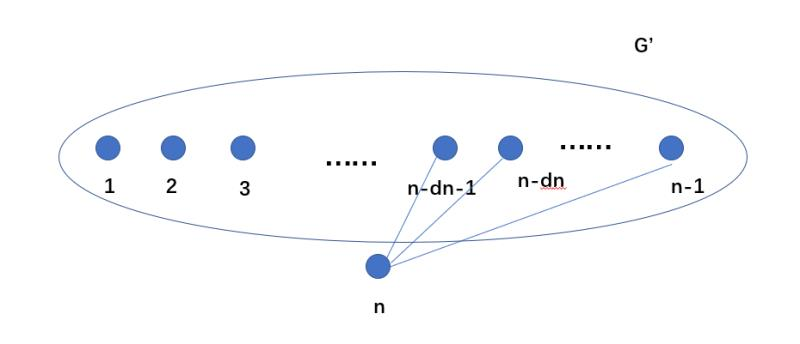
\includegraphics[width = 0.8 \textwidth]{score.png}
\end{center}
\end{figure}
%%%%%%%%%%%%%%%%%%%%%%%%%%%%%%%%%%%%%%%%%%
\par
\textbf{(4)Difficulty}
\par First, figure out what are you going to prove. The algorithm is too detailed to prove, so you must transfer it to an abstract and concise form. In fact, the algorithm works by removing some vertices and edges recursively. Similarly, we can prove by recursion, which means that we should prove d is possible only if d' is possible.
\begin{figure}[hpbt]
\begin{center}
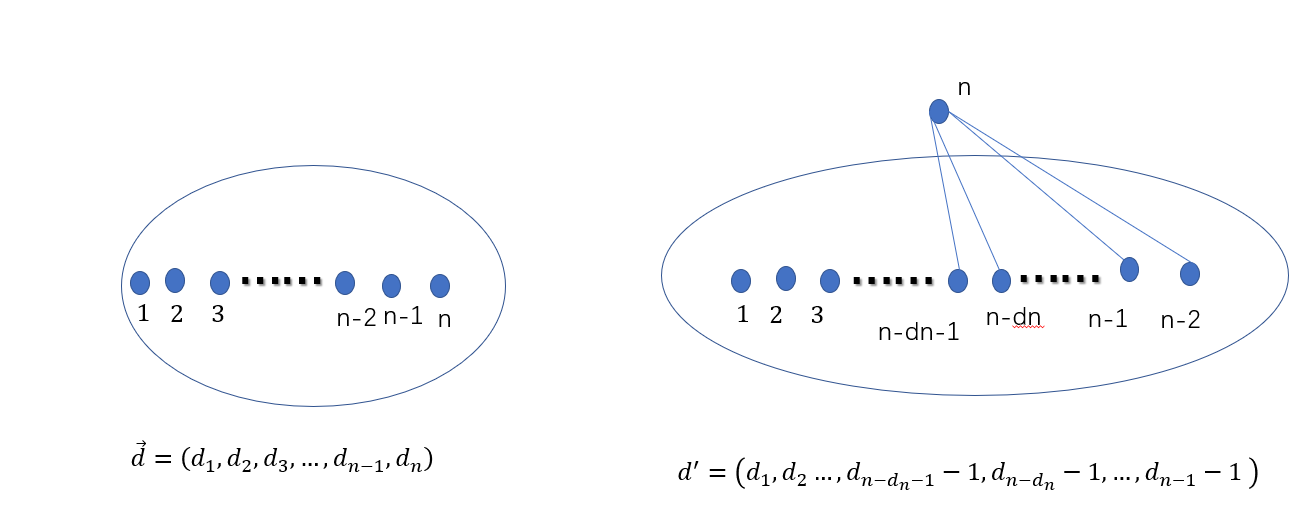
\includegraphics[width = 0.8 \textwidth]{ex1_4_1.png}
\end{center}
\end{figure}
\par Secondly, how to prove the claim d' is possible when d is possible. Obviously, a special G with d score such like the above is easy to derive, but how about other graphs? It's a challenge to transform a graph to the special G with score unchanged.It's very skilful for you to perform several operations like adding or removing some edges between some special vertices with score unchanged.After that, a graph will change to G. 
\begin{figure}[hpbt]
\begin{center}
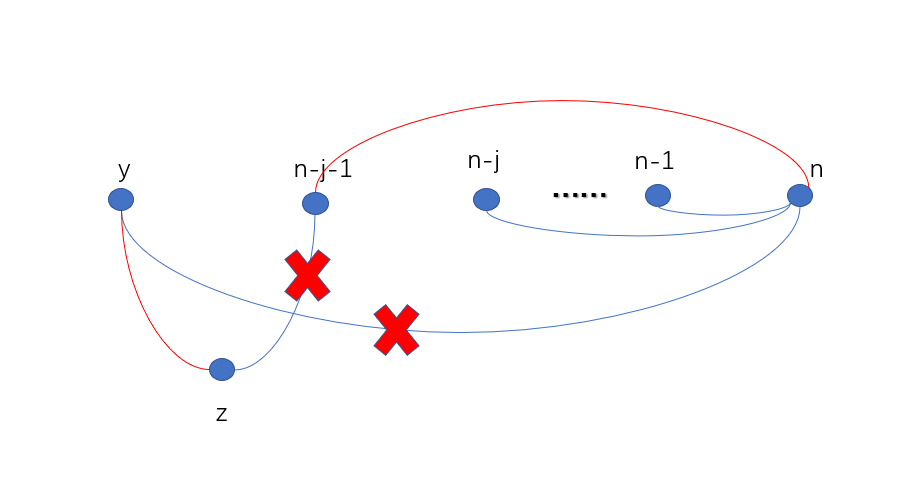
\includegraphics[width = 0.8 \textwidth]{ex1_4_2.png}
\end{center}
\end{figure}

